\documentclass{beamer}

\usetheme{Madrid}      % 内置主题(推荐新手使用)
\useoutertheme{miniframes} % 外层主题:横向小方块目录条
% \usetheme{Frankfurt}
% \usepackage[x11names]{xcolor}  % 加载扩展色库
% \usecolortheme[named=OliveDrab3]{structure}  % 柔和绿色
\usepackage{graphicx}
\usepackage{amsmath}
\usepackage{caption}

\title{Wavelet Transform for Image Processing}
\author{
\texorpdfstring{
Zhang Jinrui\thanks{alternative email:zhangjr1022@mails.jlu.edu.cn}
\\
He Jiashun
\\
Meng Jingyuan
\\
Jiang Zishen
\\
Mo Zian
}
{
Zhang Jinrui\thanks{alternative email:zhangjr1022@mails.jlu.edu.cn}
,
He Jiashun
,
Meng Jingyuan
,
Jiang Zishen
,
Mo Zian
}
}
\date{\today}

\begin{document}

\frame{\titlepage}  % 首页封面

\section{Pre-Processing}
% 步骤 1:图像加载与灰度转换
\begin{frame}{1. Image Loading and Grayscale Conversion}
    \begin{block}{Step Explanation}
        The image is loaded using a Python imaging library and converted to grayscale. \\
        This reduces data complexity and focuses analysis on structural content.
    \end{block}

    \vspace{0.5cm}
    \begin{columns}
        \column{0.5\textwidth}
        \centering
        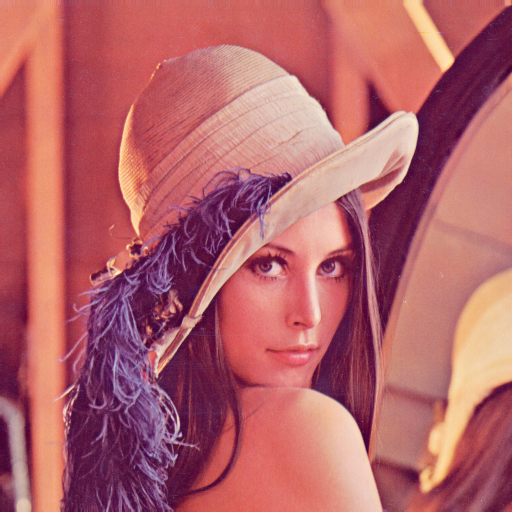
\includegraphics[width=\linewidth]{fig/lena.jpg}
        \captionof{figure}{Original Color Image}

        \column{0.5\textwidth}
        \centering
        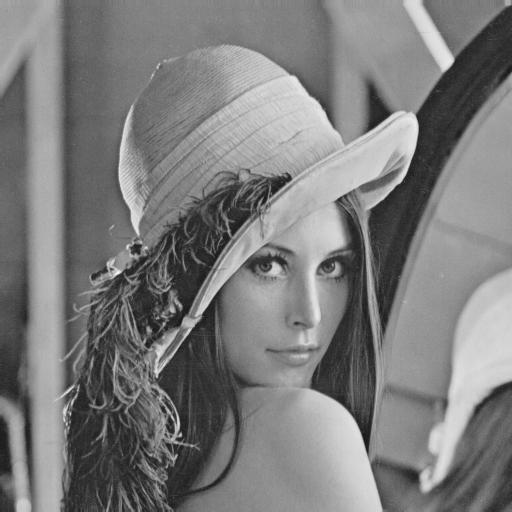
\includegraphics[width=\linewidth]{fig/gray.jpg}
        \captionof{figure}{Grayscale Converted Image}
    \end{columns}
\end{frame}

% 步骤 2 和 3:缩放和居中裁剪
\begin{frame}{2. Rescaling and 3. Centered Cropping}
    \begin{block}{Rescaling with Aspect Ratio Preservation}
        The image is resized using high-fidelity interpolation to ensure one side reaches the target length ($2^N$), without distortion. \\
        The resized image is cropped to $2^N \times 2^N$, ensuring input uniformity without compromising important visual features.
    \end{block}

    \vspace{0.3cm}
    \begin{columns}
        \column{0.5\textwidth}
        \centering
        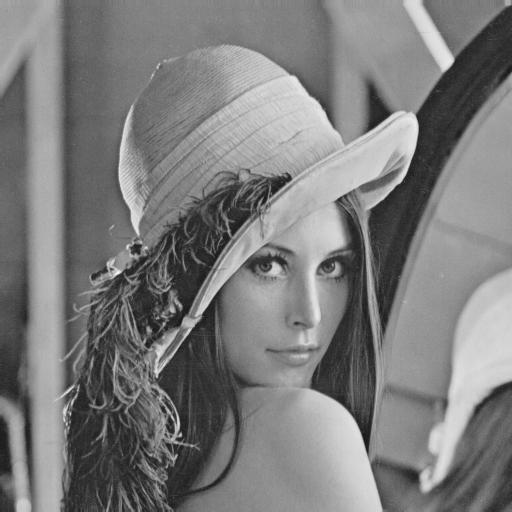
\includegraphics[width=\linewidth]{fig/gray.jpg}
        \captionof{figure}{Before Rescaling}

        \column{0.5\textwidth}
        \centering
        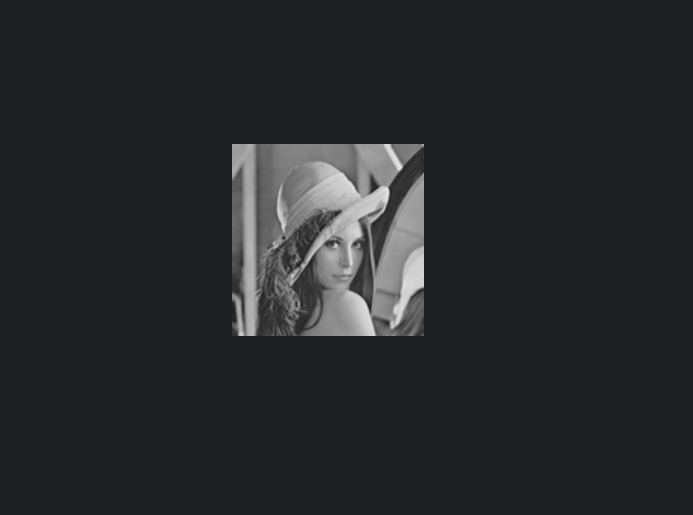
\includegraphics[width=\linewidth, height=5cm]{fig/shuoxiao.png}
        \captionof{figure}{After Rescaling ($2^N$ Side)}
    \end{columns}
\end{frame}

% 步骤 4:矩阵输出
\begin{frame}{4. Matrix Output}
    \begin{block}{Step Explanation}
        The final image is converted into a matrix format suitable for: \\
        $\boldsymbol{\cdot}$ Mathematical operations (e.g., wavelet transforms) \\
        $\boldsymbol{\cdot}$ Storage and machine learning integration
    \end{block}

    \vspace{1cm}
    \centering
    \begin{tabular}{|c|c|c|}
        \hline
        128 & 135 & 142 \\
        \hline
        130 & 138 & 145 \\
        \hline
        125 & 132 & 139 \\
        \hline
    \end{tabular} \\
    \vspace{0.5cm}
    \small{Example of 3x3 image matrix (simplified)}
\end{frame}

% 步骤 5:从矩阵还原图像
\begin{frame}{5. Convert Matrix Information into an Image}
    \begin{block}{Concept}
        Each matrix element represents the gray value of a pixel. Using this matrix, we can reconstruct the grayscale image.
    \end{block}

    \vspace{0.3cm}
    \begin{columns}
        \column{0.5\textwidth}
        \centering
        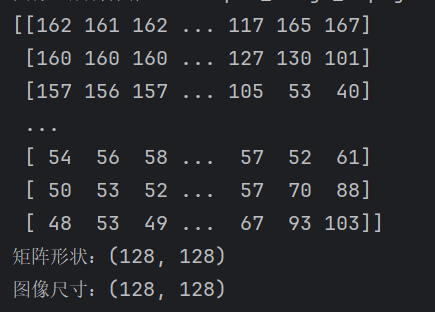
\includegraphics[width=\linewidth]{fig/matrix_information.png}
        \captionof{figure}{Matrix Information}

        \column{0.5\textwidth}
        \centering
        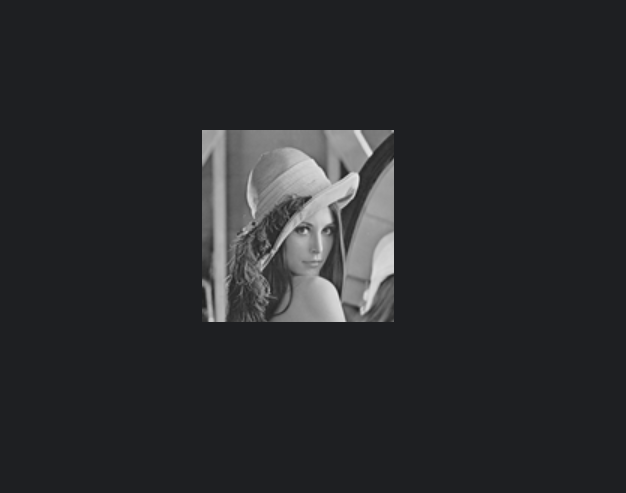
\includegraphics[width=\linewidth]{fig/The_corresponding_image.png}
        \captionof{figure}{Reconstructed Image}
    \end{columns}
\end{frame}

\section{Image compression}
\begin{frame}
    \frametitle{Image compression}
    Let's see an application of our research first.\\ \ \\
    By our research, $\forall\ m \in \mathbb{N}_{+}$, we can get \textbf{an set of orthonormal bases} of $\mathbb{R}^{m}$ quickly.
    \begin{block}{Theorem 2.1}
        Let $\{u_{i}\}_{i=1}^{m}$ is a set of \textbf{orthonormal bases} of $\mathbb{R}^{m}$, $\{v_{i}\}_{i=1}^{n}$ is a set of \textbf{orthonormal bases} of $\mathbb{R}^{n}$, then
        $$\{u_{i}\times v_{j}\ |\ i = 1,\cdots m, j=1,\cdots n\}$$
        is a set of \textbf{orthonormal bases} of $\mathbb{R}^{m\times n}$.
    \end{block}
\end{frame}
\begin{frame}
    \frametitle{Image compression}
    A grayscale image is stored as a grayscale matrix in the computer. Then we only need to know how to "{\color{blue}compress}" a matrix.\\ \ \\
    For $A \in \mathbb{R}^{m\times n}$, if $\{u_{i}\},\{v_{j}\}$ are sets of \textbf{orthonormal bases} of $\mathbb{R}^{m}$ and $\mathbb{R}^{n}$, according to (\textit{Theorem 2.1}),
    $\exists\ \omega_{i,j}\in\mathbb{R}, i = 1, \cdots m, j = 1, \cdots, n,$
    $$	A = \sum_{i,j}\omega_{i,j}\ \cdot \ u_{i} \cdot v_{j}^{T}.$$
    Let $M = (u_{1},u_{2},\cdots,u_{m}),\ N = (v_{1},v_{2},\cdots,v_{n}), W = (\omega_{i,j}).$ Then
    $$M^{T}AN =W,\ MWN^{T} = A.$$
\end{frame}
\begin{frame}
    \frametitle{Image compression}
    {\color{red}If $\omega_{i,j}$ is too small, the influence of  corresponding basis can be ignored.} \\Then
    \begin{align*}
        \widetilde{A} = \sum_{i,j}\widetilde{\omega_{i,j}}\ \cdot \ u_{i} \cdot v_{j}^{T},\ \widetilde{\omega_{i,j}} = \left\{
        \begin{aligned}
             & \omega_{i,j}, & \ |\omega_{i,j}| > \lambda    \\
             & 0,            & \ |\omega_{i,j}| \leq \lambda
        \end{aligned}
        \right..
    \end{align*}
    $\widetilde{A}$ is an approximation of $A$, while $\lambda$ is image compression strength.\\ \ \\
    Let $\widetilde{W} = (\widetilde{\omega_{i,j}}).$ As long as $\lambda$ is large enough, we can transform $\widetilde{W}$ into a \textbf{sparse matrix} which needs less storage space.\\ \ \\
    {\color{blue}Then we set $\lambda$ equal to $0.5$ and see the result.}
\end{frame}
\begin{frame}
    \frametitle{Image compression}
    \begin{figure}[ht!]
        \centering
        \begin{minipage}{0.45\textwidth}
            \centering
            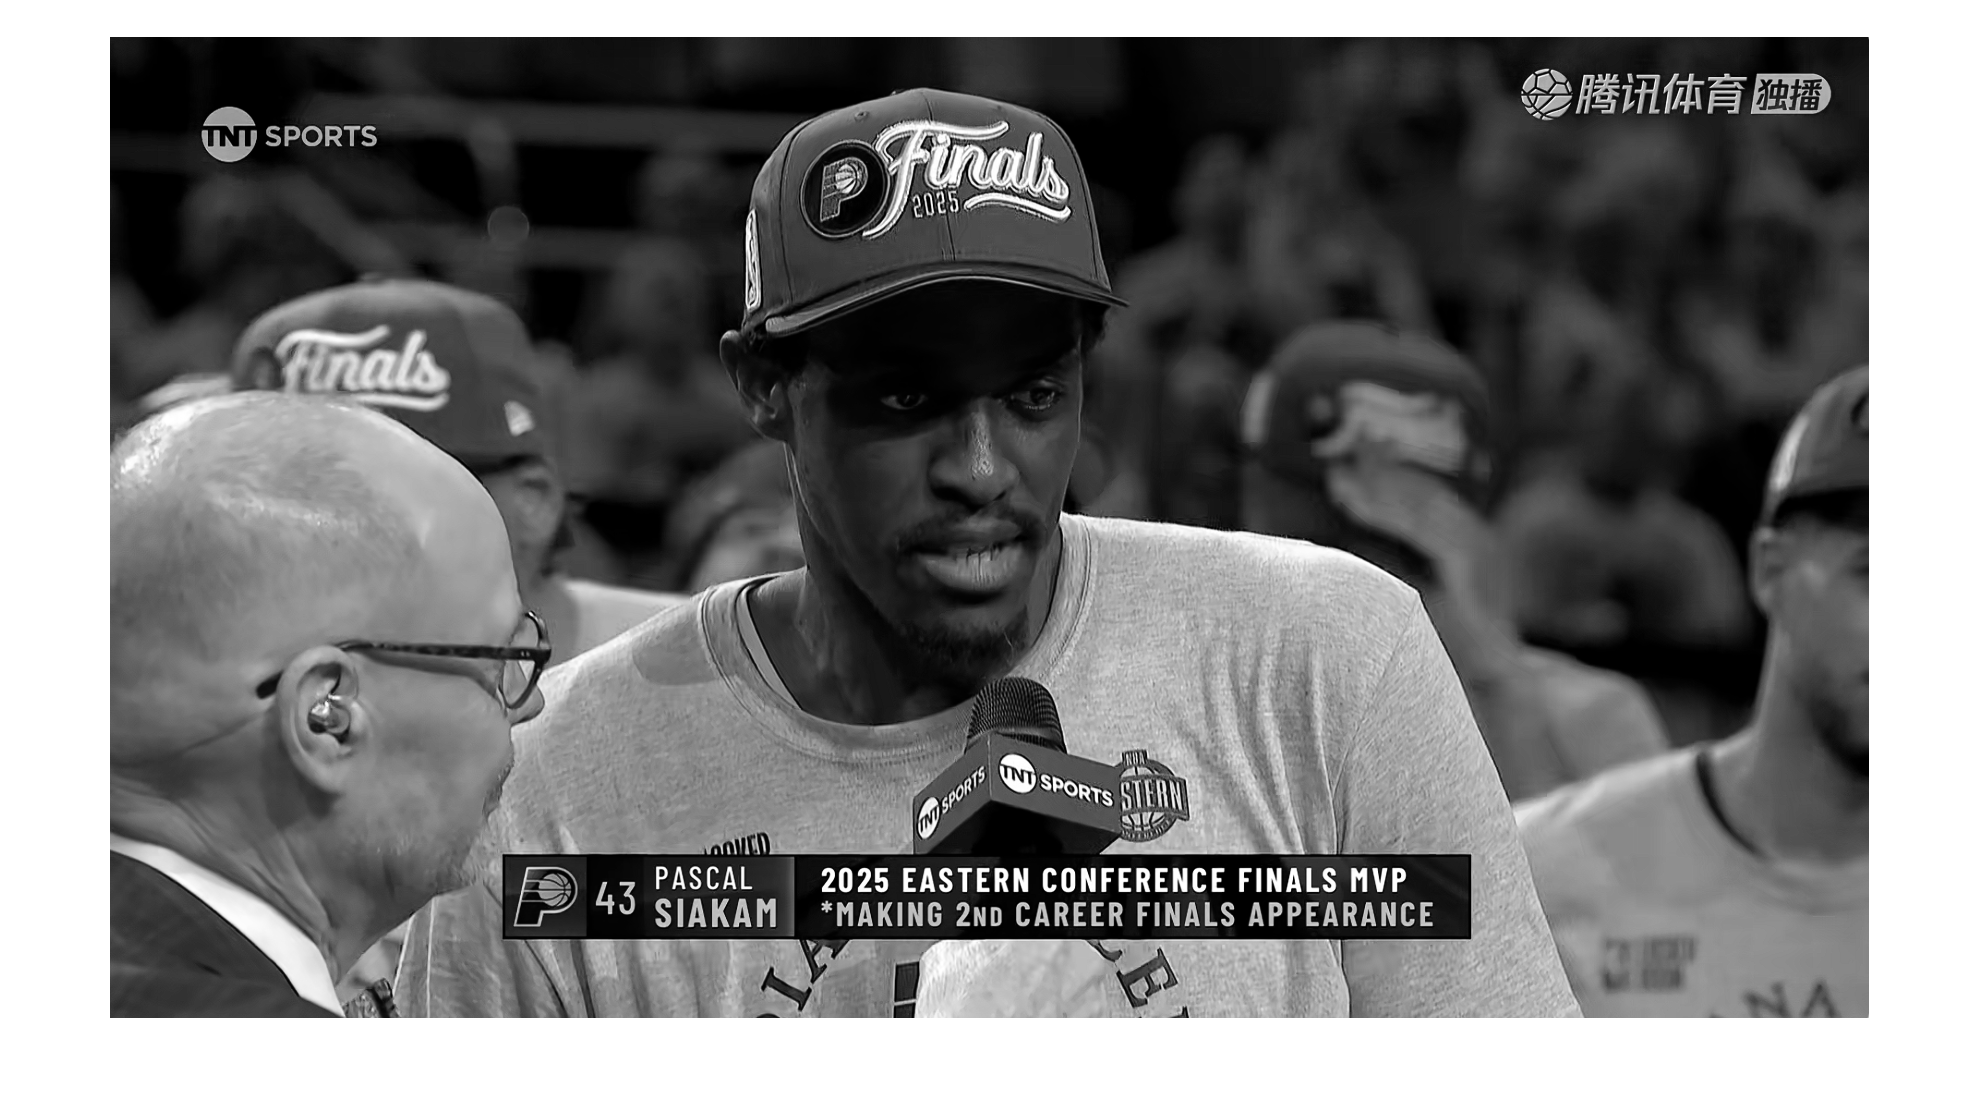
\includegraphics[width=0.9\textwidth]{fig/Siakam_gray.png} % first figure itself
            \caption{Original image}
            % \label{fig:Haar_sin}
        \end{minipage}\hfill
        \begin{minipage}{0.45\textwidth}
            \centering
            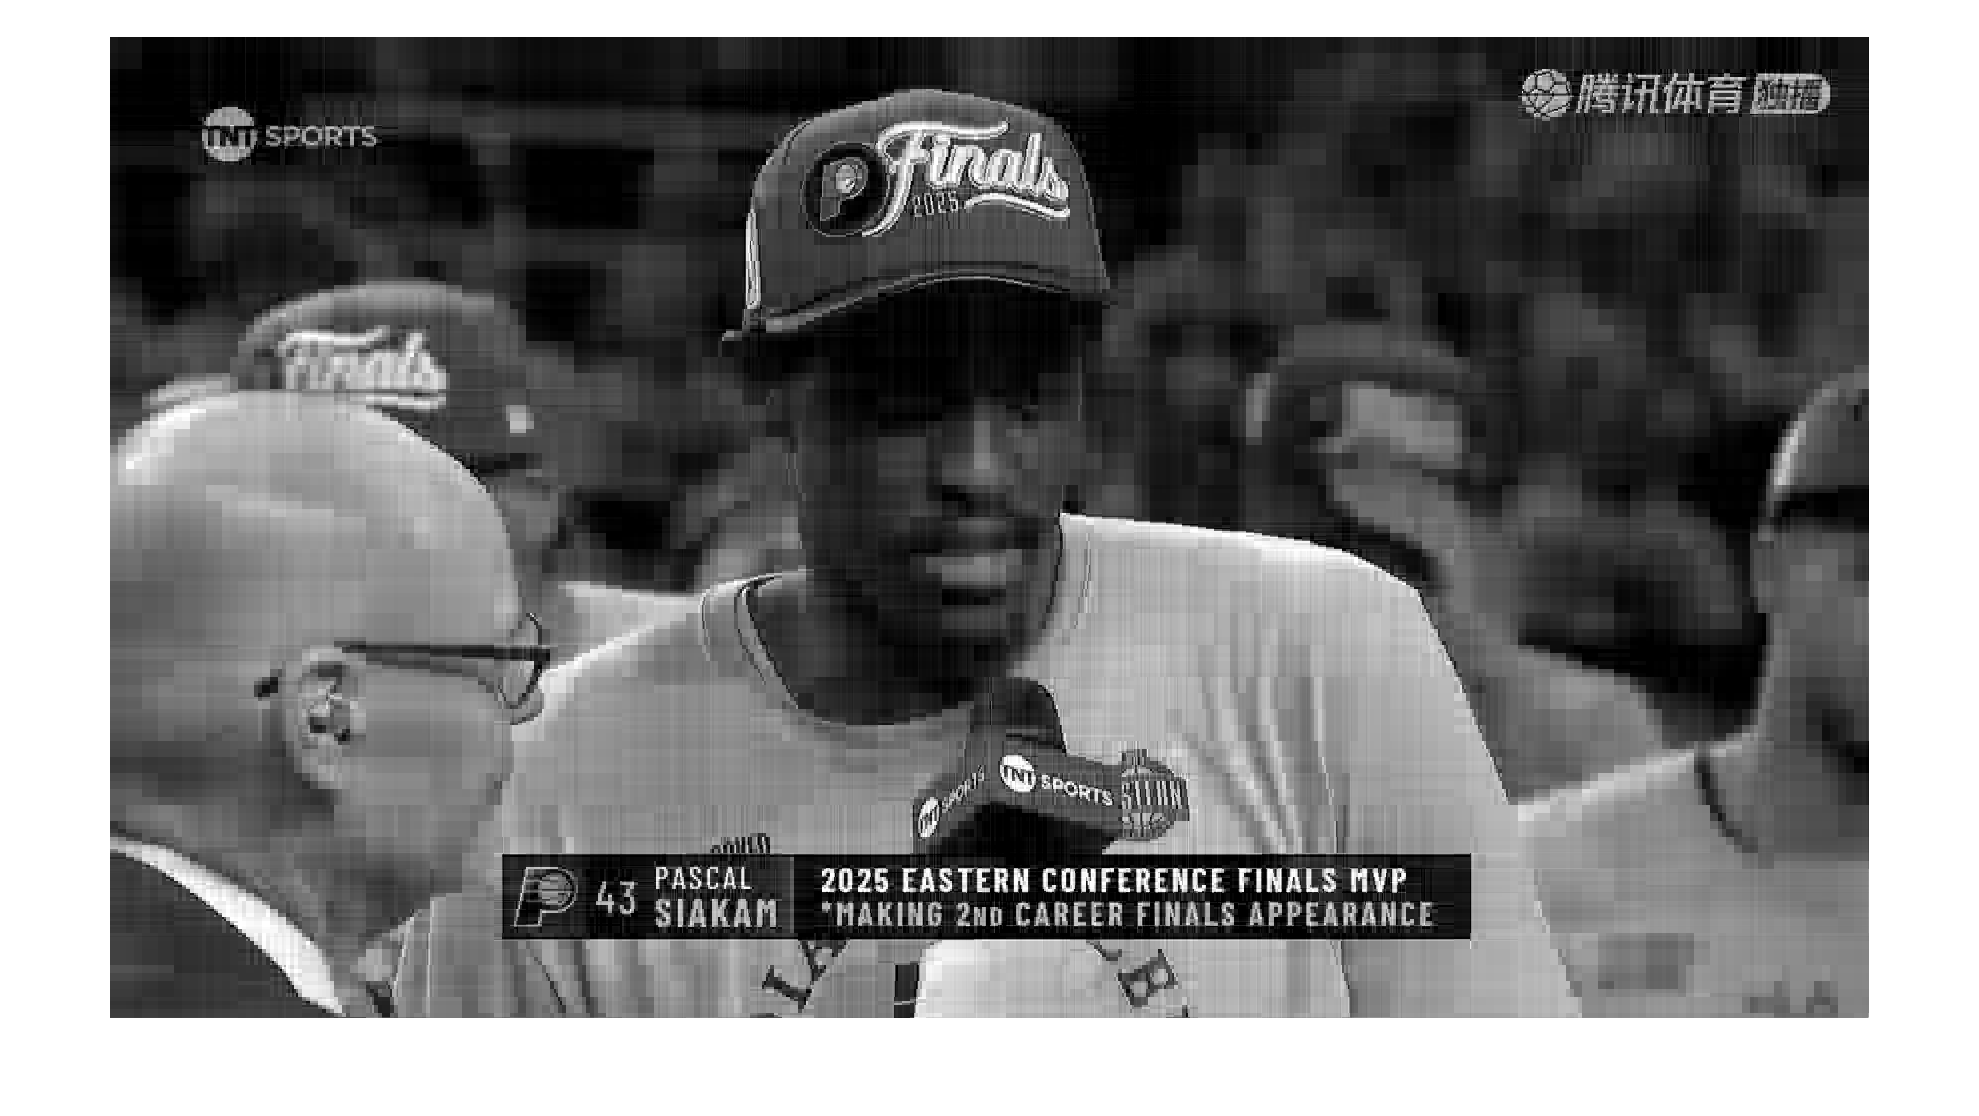
\includegraphics[width=0.9\textwidth]{fig/Siakam_compressed.png} % second figure itself
            \caption{Final image}
        \end{minipage}
    \end{figure}
\end{frame}
\begin{frame}
    \frametitle{Image compression}
    For original image , the size of stored information is $981\times1759 = 1725579$. \\\ \\
    {\color{red} However, after compression, the size of stored information is  only $15364\times2 = 30728$.} \\\ \\
    Indeed, we reduce storage space by compression. However, we also lose much detailed information of original picture. That's why we should change $\lambda$ for different purposes to reach the balance.
\end{frame}

\section{Energy Conservation}
% \subsection{Research background and objectives}

\begin{frame}{Research background and objectives}
    \begin{block}{Advantages of Wavelet Transform}
        - Multiresolution analysis \\
        - frequency localization capability
    \end{block}

    \begin{block}{Importance of Energy Conservation}
        - Ensures information integrity in signal processing  \\
        - Theoretical basis for image compression, denoising
    \end{block}

    \begin{block}{Research Objectives}
        - Validate energy conservation mathematically  \\
        - Quantify energy retention via image compression experiments
    \end{block}
\end{frame}

% \subsection{Theoretical analysis}


\begin{frame}{Theoretical analysis}
    \begin{block}{Theoretical Foundations of DWT}
        \begin{itemize}
            \item Scaling function ($\phi$) and wavelet function ($\psi$)
            \item Multi-scale decomposition: Approximation ($cA$) and Detail   ($cH$, $cV$, $cD$) subbands
            \item Orthogonal Wavelet Basis Properties:
                  \[
                      \langle \psi_{j,k},\,\psi_{m,n}\rangle
                      = \delta_{j,m}\,\delta_{k,n},
                      \qquad j,k,m,n\in\mathbb{Z}
                  \]


        \end{itemize}
    \end{block}





    \begin{block}{Critical Conditions}
        \begin{itemize}
            \item Use of orthogonal wavelets (e.g., Haar, Db1)
            \item No signal truncation or padding-induced errors
        \end{itemize}
    \end{block}
\end{frame}
\begin{frame}{ Energy Conservation Formula }
    \begin{block}{Energy Conservation Formula for Orthogonal DWT}
        \begin{itemize}
            \item For orthogonal wavelet bases:
                  \[
                      \sum_{i=1}^{M} \sum_{j=1}^{N} |x[i,j]|^2 = \sum_{k,l} |d_k[l]|^2 + \sum_{m} |a_J[m]|^2
                  \]
            \item For Haar wavelet bases:

                  \[
                      \begin{aligned}
                          \sum_{i,j} |x[i,j]|^2 =\sum_{i,j} |cA[i,j]|^2 + \sum_{i,j} |cH[i,j]|^2 \\+ \sum_{i,j} |cV[i,j]|^2 +\sum_{i,j} |cD[i,j]|^2
                      \end{aligned}
                  \]
        \end{itemize}
    \end{block}



\end{frame}
% \subsection{Experimental Design and Code Implementation}

\begin{frame}{Experimental Design and Code Implementation}
    \begin{block}{Workflow}
        \begin{itemize}
            \item Image preprocessing
                  \begin{itemize}
                      \item grayscale conversion
                      \item resizing to power-of-2 dimensions
                  \end{itemize}
            \item DWT decomposition("dwt2"function)
            \item Energy calculation and conservation validation
            \item Image reconstruction("idwt2"function)
        \end{itemize}
    \end{block}
    \begin{block}{Parameters}
        \begin{itemize}
            \item Test image:"Lena"(52*52)
            \item Wavelet basis:Haar
        \end{itemize}
    \end{block}

\end{frame}

\begin{frame}{Code and Implementation}
    \begin{figure}
        \centering
        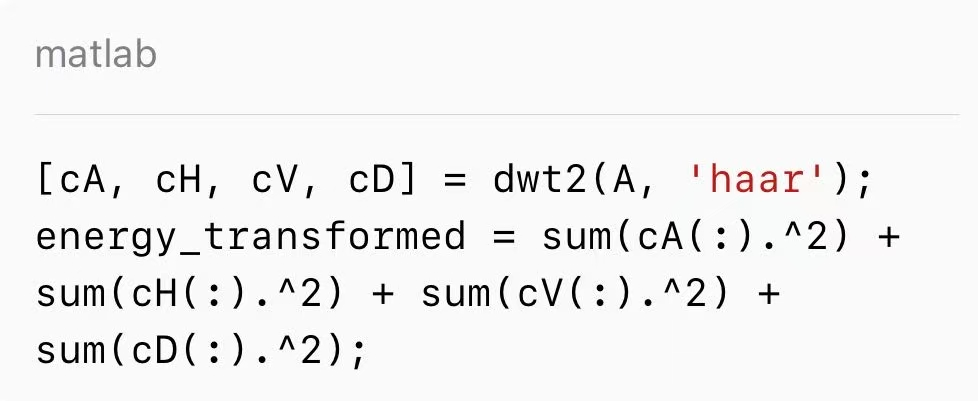
\includegraphics[width=0.5\linewidth]{fig/代码2.jpg}
        \caption{"Haar"basis}
        % \label{fig:placeholder}
    \end{figure}
    \begin{figure}
        \centering
        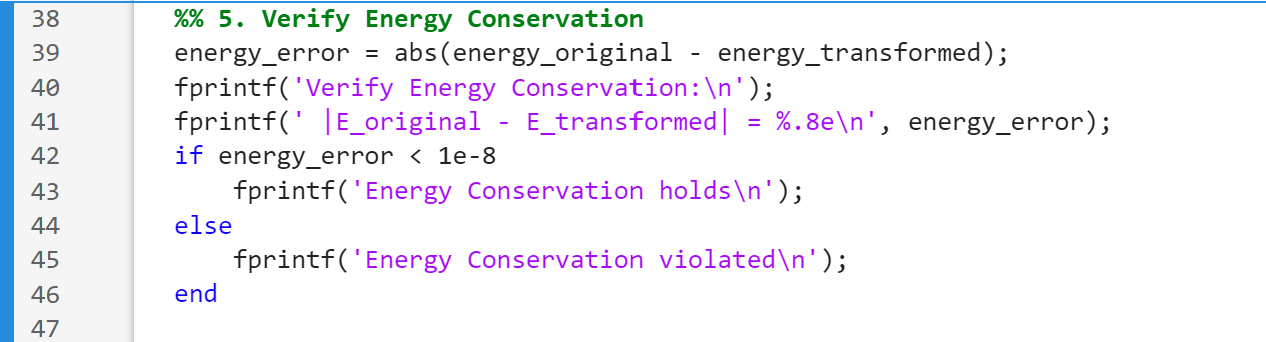
\includegraphics[width=1\linewidth]{fig/代码3.png}
        \caption{Verify Energy Conservation}
        % \label{fig:placeholder}
    \end{figure}
\end{frame}


\begin{frame}{Code and Implementation}
    \begin{figure}
        \centering
        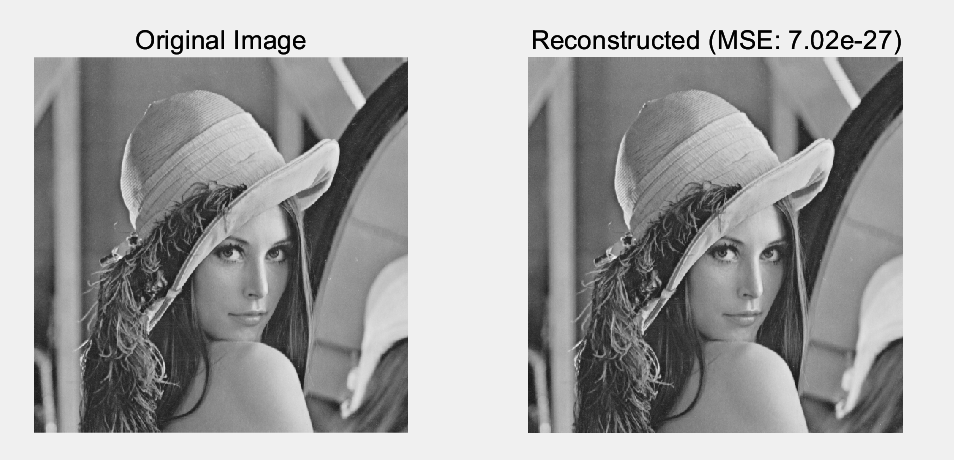
\includegraphics[width=0.5\linewidth]{fig/图像1.png}

        % \label{fig:placeholder}
    \end{figure}

    \begin{figure}
        \centering
        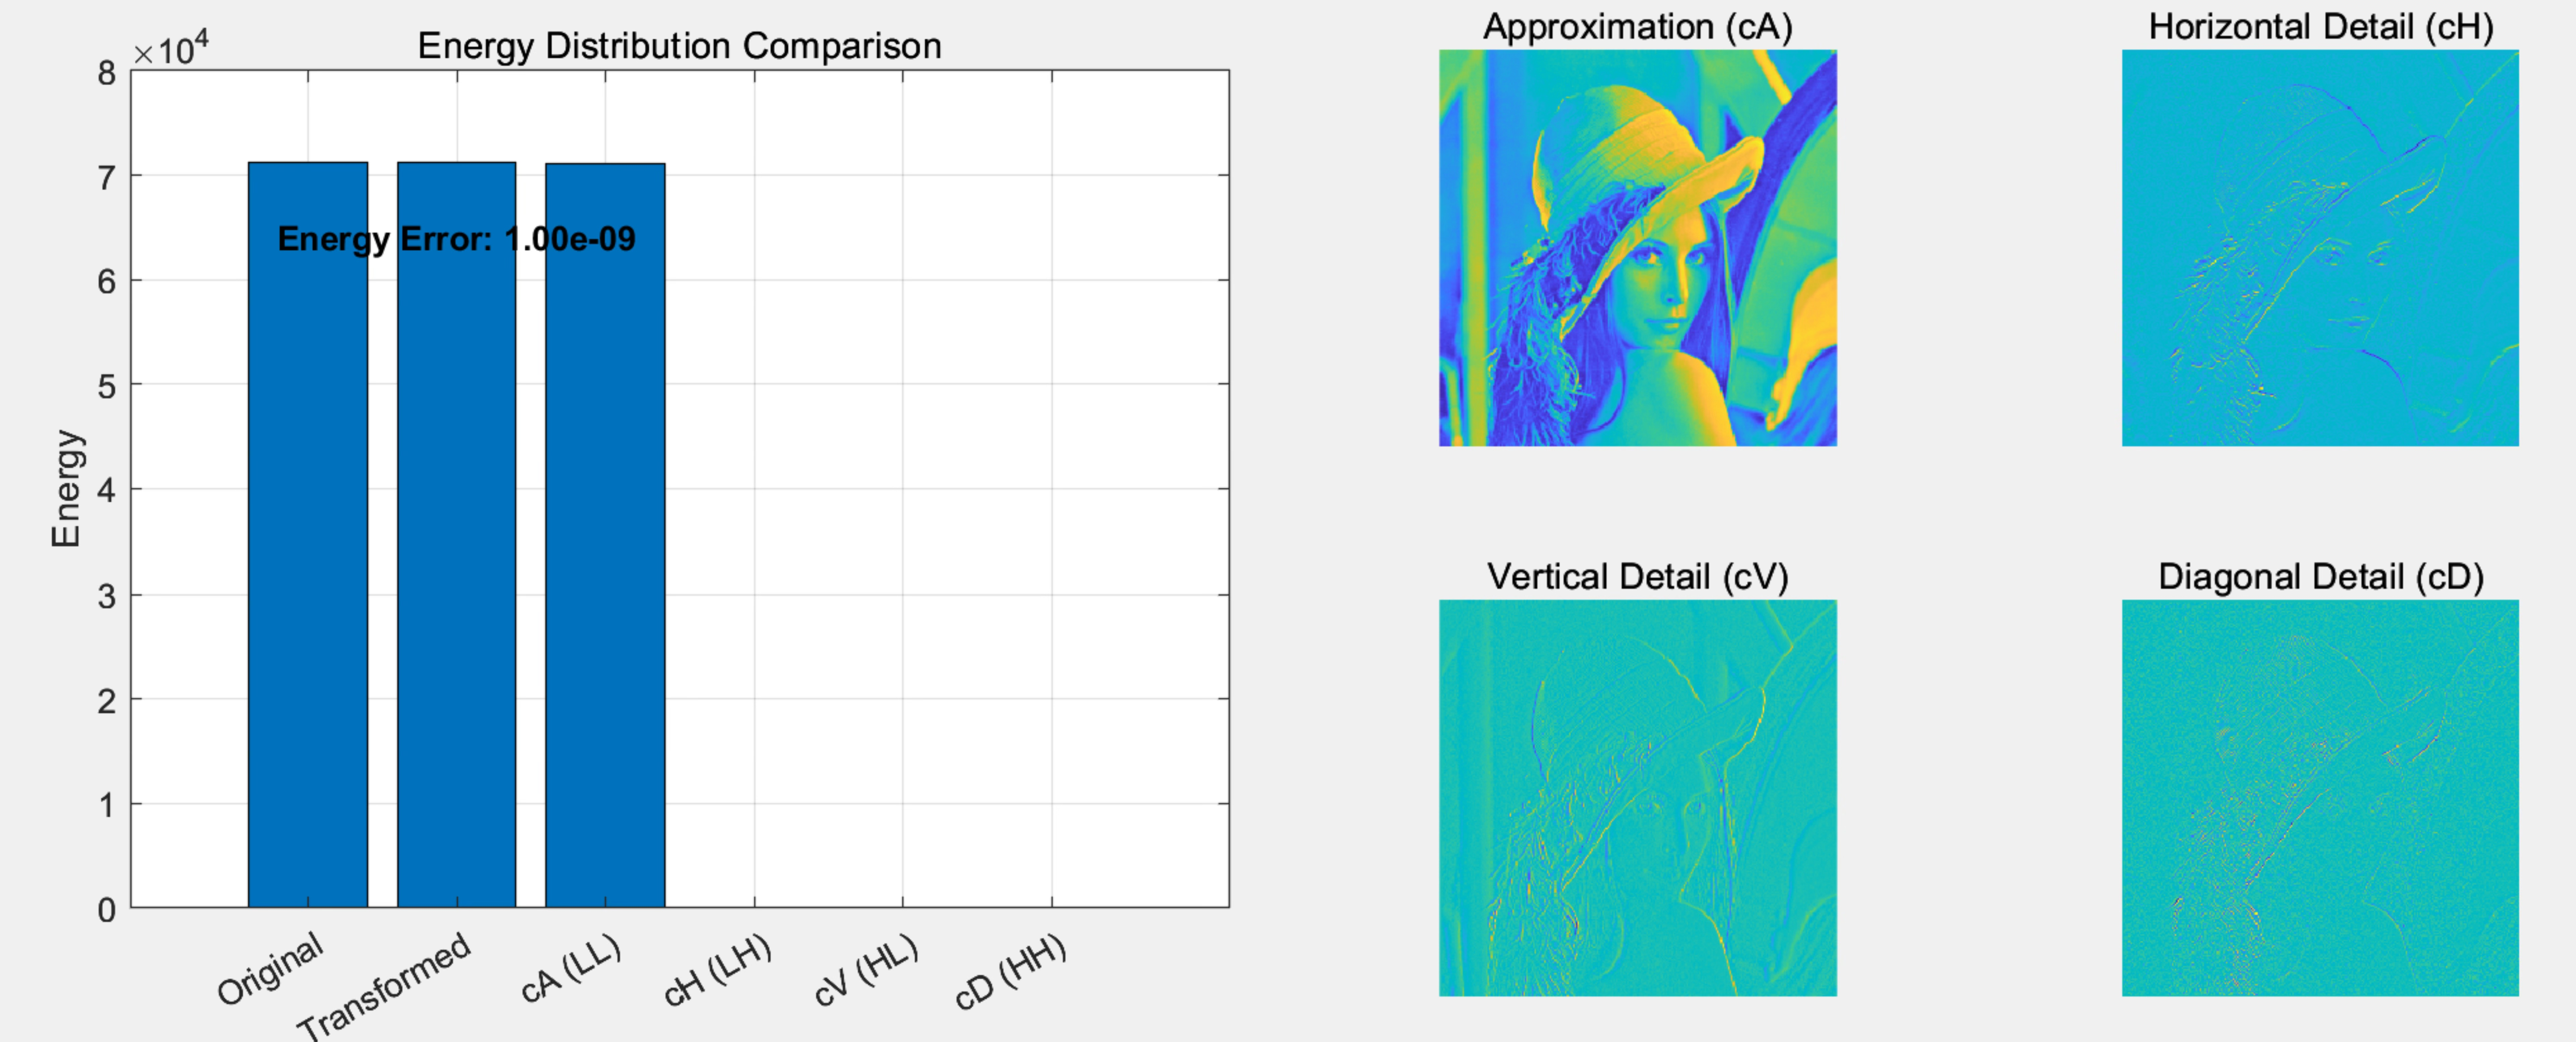
\includegraphics[width=0.75\linewidth]{fig/图片4.jpg}

        % \label{fig:placeholder}
    \end{figure}
\end{frame}

% \subsection{Conclusions and Future Work}
% \begin{frame}{Conclusions and Future Work}
%     \begin{block}{Conclusions}
%         \begin{itemize}
%             \item DWT strictly satisfies energy conservation when using orthogonal wavelet bases
%             \item Proper image size alignment and orthogonal basis selection are critical factors
%         \end{itemize}
%     \end{block}
%     \begin{block}{Future Work}
%         \begin{itemize}
%             \item Energy error analysis for non-orthogonal wavelet frames
%             \item Study of energy distribution in multi-scale decomposition (multi-level DWT)
%         \end{itemize}
%     \end{block}

% \end{frame}

\section{Augmented compression}
\begin{frame}
    \frametitle{Basic Idea}
    \begin{itemize}
        \item \[
                  \Big(\frac{\sum_{k=1}^{n}\hat{l}_k}{n}\Big)^2\;\le\;\frac{\sum_{k=1}^{n}\hat{l}_k^2}{n}.
              \]
        \item \[
                  \sum_{k=1}^{n}\hat{l}_k^4
                  \geq
                  \frac{(\sum_{k=1}^{n}\hat{l}_k^2)^2}{n}
                  =
                  \frac{(\sum_{k=1}^{n}l_k^2)^2}{n}
              \]
        \item \[
                  \min_{\hat{l}_k\in l^2 st. \sum_{k=1}^{n}\hat{l}_k^2=\sum_{k=1}^{n}l_k^2}(-\sum_{k=1}^{n}\hat{l}_k^4)
              \]
    \end{itemize}
\end{frame}
\begin{frame}
    \frametitle{Basic Idea}
    \begin{itemize}
        \item 	\begin{figure}
                  \centering
                  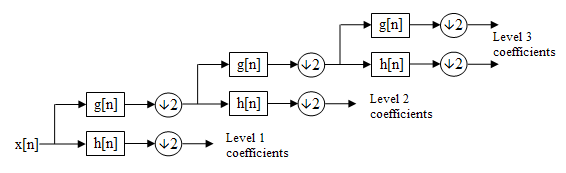
\includegraphics[width=0.8\textwidth]{fig/Wavelets_-_Filter_Bank.png}
                  \caption{Cascading}
                  \label{fig:Cascading}
              \end{figure}
        \item \[
                  \min_{\Phi}(-\sum_{k=1}^{n}\hat{l}_k^4)
              \]
        \item Condense the energy to as less coefficients as possible.
    \end{itemize}
\end{frame}
\begin{frame}
    \frametitle{Results}
    \begin{itemize}
        \item
              \begin{figure}[ht!]
                  \centering
                  \begin{minipage}{0.45\textwidth}
                      \centering
                      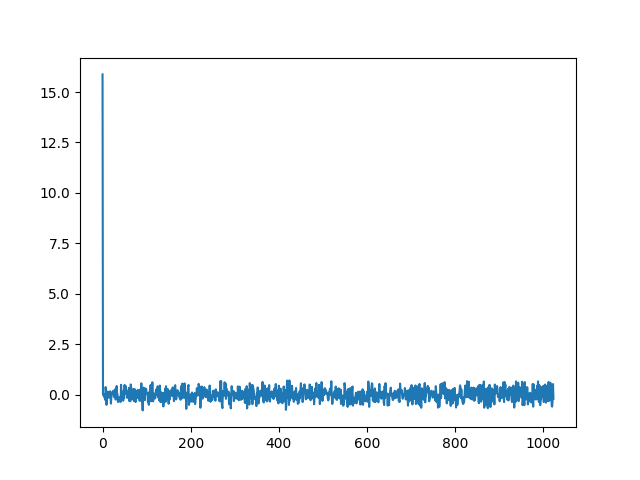
\includegraphics[width=0.9\textwidth]{fig/HaarAugmented1D_freq.png} % first figure itself
                      \caption{Haar 2x2 filter bank random input. Compression Rate 0.2568}
                      \label{fig:Haar}
                  \end{minipage}\hfill
                  \begin{minipage}{0.45\textwidth}
                      \centering
                      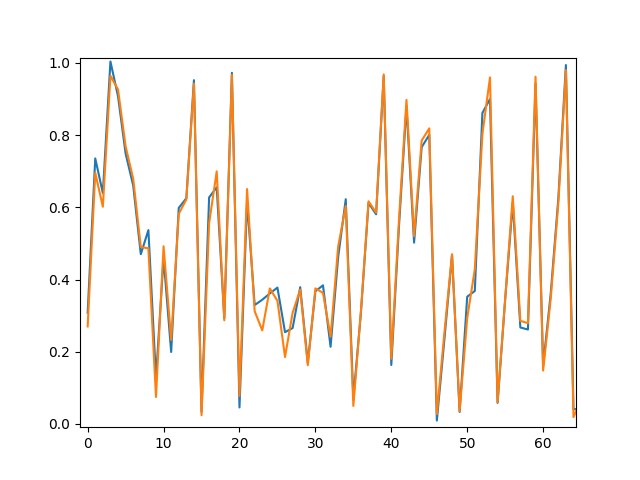
\includegraphics[width=0.9\textwidth]{fig/HaarAugmented1D_rec.png} % second figure itself
                      \caption{Haar 2x2 filter bank random input.Total average energy loss 0.0009}
                  \end{minipage}
              \end{figure}
              %   \begin{figure}
              %       \centering
              %       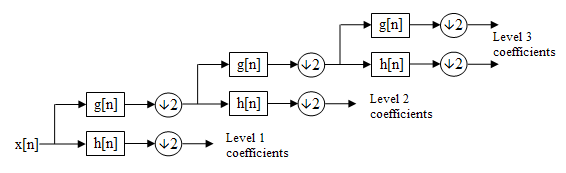
\includegraphics[width=0.8\textwidth]{fig/Wavelets_-_Filter_Bank.png}
              %       \caption{Siakam won 2025 NBA eastern conference finals MVP}
              %       \label{fig:Siakam}
              %   \end{figure}
              % \item Random sequence would have large information entropy so it have a low compression rate.
    \end{itemize}
\end{frame}
\begin{frame}
    \frametitle{Results}
    \begin{itemize}
        \item
              \begin{figure}[ht!]
                  \centering
                  \begin{minipage}{0.45\textwidth}
                      \centering
                      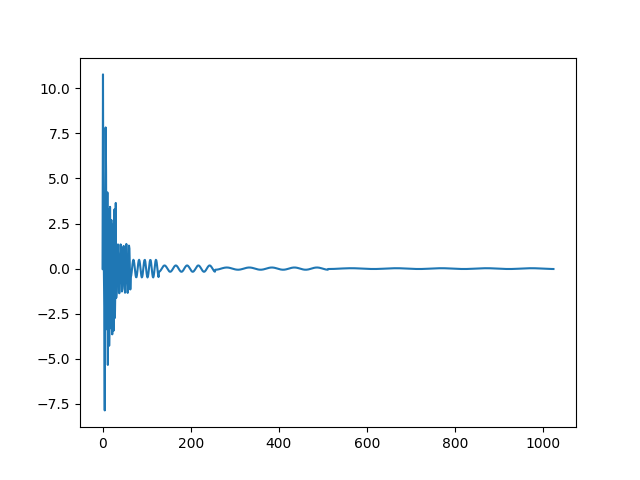
\includegraphics[width=0.9\textwidth]{fig/HaarAugmented1D_sin_freq.png} % first figure itself
                      \caption{Haar 2x2 filter bank sin input frequency. Compression Rate 0.9287}
                      \label{fig:Haar_sin}
                  \end{minipage}\hfill
                  \begin{minipage}{0.45\textwidth}
                      \centering
                      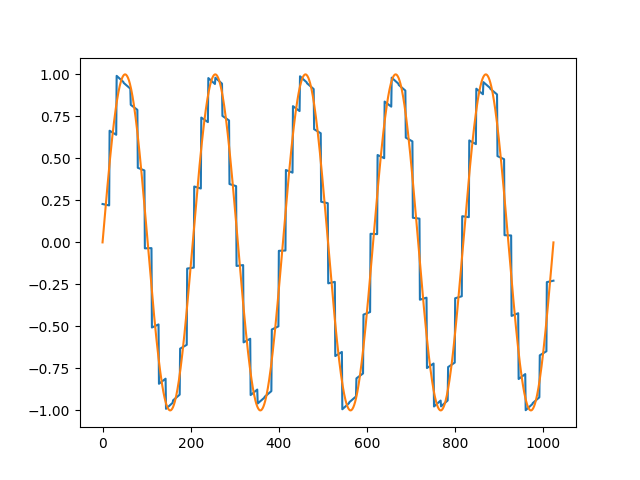
\includegraphics[width=0.9\textwidth]{fig/HaarAugmented1D_sin_rec.png} % second figure itself
                      \caption{Haar 2x2 filter bank sin input reconstruction.Total average energy loss 0.0104}
                  \end{minipage}
              \end{figure}
              %   \begin{figure}
              %       \centering
              %       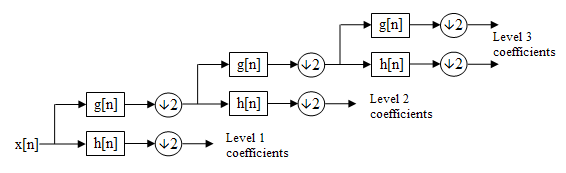
\includegraphics[width=0.8\textwidth]{fig/Wavelets_-_Filter_Bank.png}
              %       \caption{Siakam won 2025 NBA eastern conference finals MVP}
              %       \label{fig:Siakam}
              %   \end{figure}
              % \item A smooth signal have small information entropy, so will have a high compression rate.
    \end{itemize}
\end{frame}
\begin{frame}
    \frametitle{Results}
    \begin{itemize}
        \item
              \begin{figure}[ht!]
                  \centering
                  \begin{minipage}{0.45\textwidth}
                      \centering
                      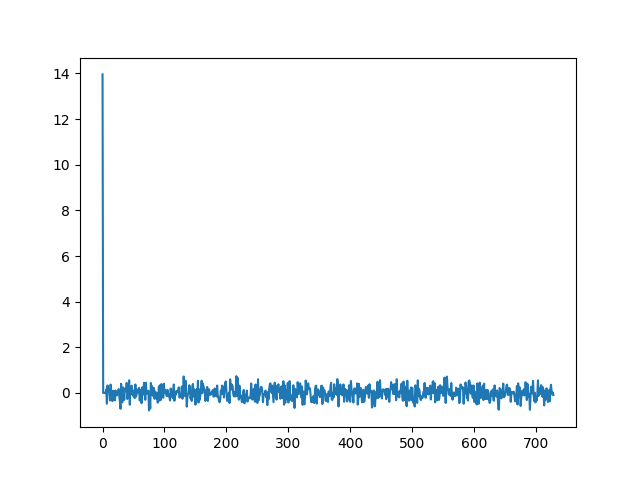
\includegraphics[width=0.9\textwidth]{fig/Haar3Augmented1D_freq.png} % first figure itself
                      \caption{Haar 3x3 filter bank random input. Compression Rate 0.1906}
                      \label{fig:Haar3}
                  \end{minipage}\hfill
                  \begin{minipage}{0.45\textwidth}
                      \centering
                      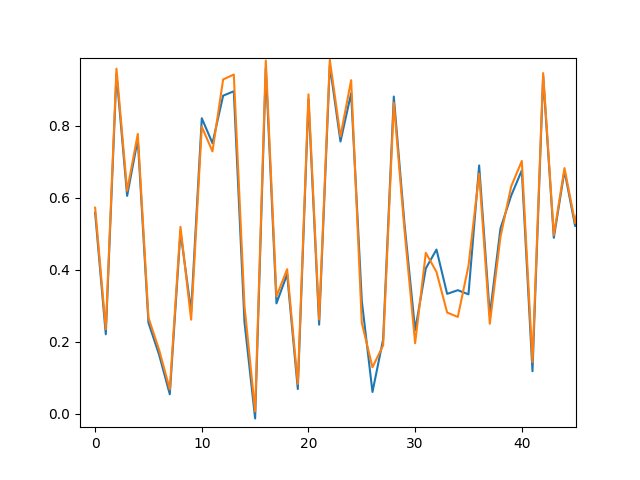
\includegraphics[width=0.9\textwidth]{fig/Haar3Augmented1D_rec.png} % second figure itself
                      \caption{Haar 3x3 filter bank random input.Total average energy loss 0.0008}
                  \end{minipage}
              \end{figure}
              %   \begin{figure}
              %       \centering
              %       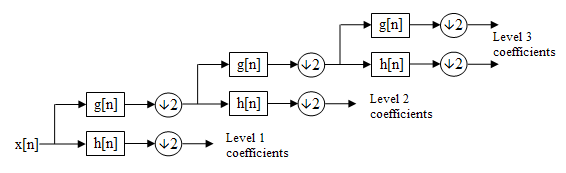
\includegraphics[width=0.8\textwidth]{fig/Wavelets_-_Filter_Bank.png}
              %       \caption{Siakam won 2025 NBA eastern conference finals MVP}
              %       \label{fig:Siakam}
              %   \end{figure}
              % \item same random sequence same reason.
    \end{itemize}
\end{frame}
\begin{frame}
    \frametitle{Results}
    \begin{itemize}
        \item
              \begin{figure}[ht!]
                  \centering
                  \begin{minipage}{0.45\textwidth}
                      \centering
                      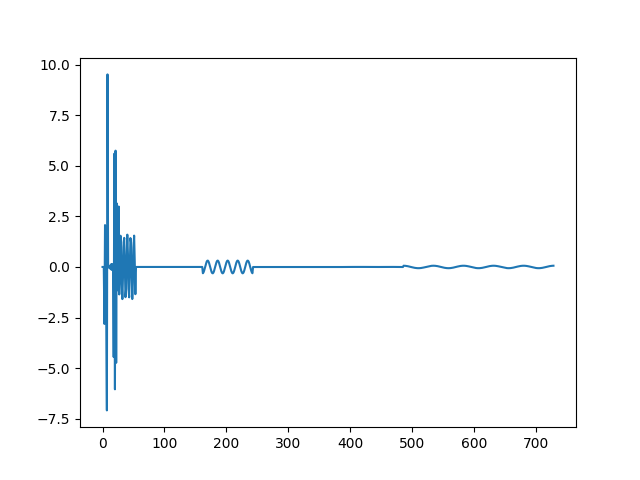
\includegraphics[width=0.9\textwidth]{fig/Haar3Augmented1D_sin_freq.png} % first figure itself
                      \caption{Haar 3x3 filter bank sin input frequency. Compression Rate 0.7750}
                      \label{fig:Haar3_sin}
                  \end{minipage}\hfill
                  \begin{minipage}{0.45\textwidth}
                      \centering
                      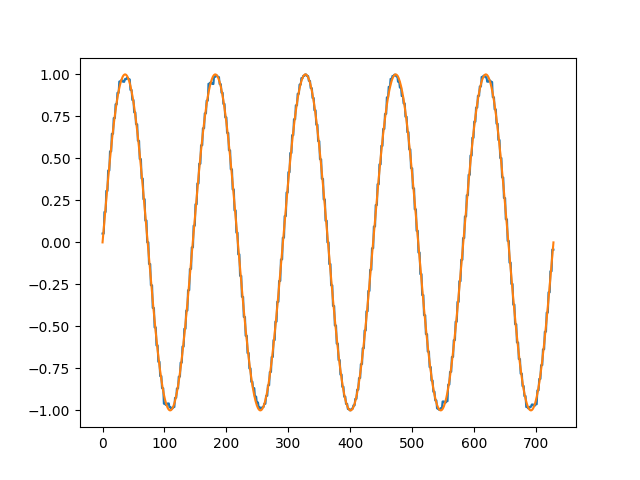
\includegraphics[width=0.9\textwidth]{fig/Haar3Augmented1D_sin_rec.png} % second figure itself
                      \caption{Haar 3x3 filter bank sin input reconstruction.Total average energy loss 0.0007}
                  \end{minipage}
              \end{figure}
              %   \begin{figure}
              %       \centering
              %       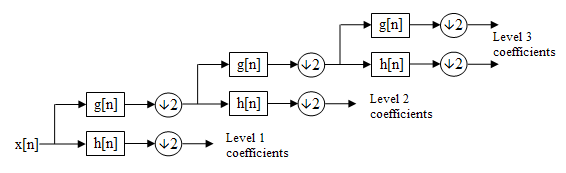
\includegraphics[width=0.8\textwidth]{fig/Wavelets_-_Filter_Bank.png}
              %       \caption{Siakam won 2025 NBA eastern conference finals MVP}
              %       \label{fig:Siakam}
              %   \end{figure}
              % \item same smooth signal same reason.
    \end{itemize}
\end{frame}

\section{Perfect Reconstruction}


\begin{frame}{Sequence Spaces}
    \begin{itemize}
        \item $\ell(\mathbb{Z})=\bigl\{v=\{v(k)\}_{k\in\mathbb{Z}}\mid v(k)\in\mathbb{C}\bigr\}$
        \item $\ell_0(\mathbb{Z})=\bigl\{u\in\ell(\mathbb{Z})\mid \text{only finitely many } u(k)\neq 0\bigr\}$
        \item filter bank: $\{u_0,\dots,u_s\}\subset \ell_0(\mathbb{Z})$
    \end{itemize}
\end{frame}


\begin{frame}{Operators}
    \begin{itemize}
        \item \textbf{Subdivision:}
              \[
                  [S_u v](n)=2\sum_{k\in\mathbb{Z}} v(k)\,u(n-2k)
              \]
        \item \textbf{Transition:}
              \[
                  [T_u v](n)=2\sum_{k\in\mathbb{Z}} v(k)\,\overline{u(k-2n)}
              \]
        \item \textbf{Discrete Framelet Transform (DFrT):}
              \[
                  \frac12\sum_{\ell=0}^{s} S_{u_\ell}T_{\tilde u_\ell}v
              \]
    \end{itemize}
\end{frame}


\begin{frame}{Perfect Reconstruction Condition}
    \begin{itemize}
        \item the transform satisfies perfect reconstruction if
              \[
                  \frac{1}{2}\sum_{\ell=0}^s S_{u_\ell} T_{\tilde{u}_\ell} v = v \quad \forall v\in\ell(\mathbb{Z}).
              \]
    \end{itemize}
\end{frame}


\begin{frame}{Main Theorem -- Four Equivalent Statements}
    The following are equivalent:

    \begin{enumerate}
        \item The filter bank $(\{\tilde u_\ell\},\{u_\ell\})$ has PR.
        \item The identity $\displaystyle\frac12\sum_{\ell=0}^{s} S_{u_\ell}T_{\tilde u_\ell}v = v$ holds for all $v\in\ell_0(\mathbb{Z})$.
        \item The identity $\displaystyle\frac12\sum_{\ell=0}^{s} S_{u_\ell}T_{\tilde u_\ell}v = v$ holds for $v=\delta$ and $v=\delta(\cdot-1)$.
        \item Frequency-domain identities for all $\omega\in\mathbb{R}$:
              \[
                  \sum_{\ell=0}^{s}\overline{\hat{\tilde u}_\ell(\omega)}\hat u_\ell(\omega)=1,
              \]
              \[
                  \sum_{\ell=0}^{s}\overline{\hat{\tilde u}_\ell(\omega)}\hat u_\ell(\omega+\pi)=0.
              \]
    \end{enumerate}
\end{frame}



\begin{frame}{(i) $\Rightarrow$ (ii) $\Rightarrow$ (iii)}
    Trivial inclusions:
    \[
        \ell_0(\mathbb{Z})\subseteq \ell(\mathbb{Z})\quad\text{and}\quad \delta,\delta(\cdot-1)\in\ell_0(\mathbb{Z}).
    \]
\end{frame}

\begin{frame}{(iii) $\Rightarrow$ (iv)}
    \begin{enumerate}
        \item \textbf{Frequency Domain Conversion:} Using Fourier transforms of $T_{\tilde{u}_\ell}$ and $S_{u_\ell}$:
              \[
                  \widehat{T_{\tilde{u}_\ell} v}(\omega) = \hat{v}(\omega/2)\overline{\hat{\tilde{u}}_\ell(\omega/2)} + \hat{v}(\omega/2+\pi)\overline{\hat{\tilde{u}}_\ell(\omega/2+\pi)},
              \]
              \[
                  \widehat{S_{u_\ell} w}(\omega) = \hat{w}(2\omega)\hat{u}_\ell(\omega).
              \]

        \item \textbf{Substitute Basis Signals:} Plugging $v = \delta$ ($\hat{v}=1$) and $v = \delta(\cdot-1)$ ($\hat{v}=e^{-i\omega}$) into the PR condition yields the system:
              \[
                  \sum_{\ell=0}^s \overline{\hat{\tilde{u}}_\ell(\omega)}\hat{u}_\ell(\omega) + \sum_{\ell=0}^s \overline{\hat{\tilde{u}}_\ell(\omega+\pi)}\hat{u}_\ell(\omega+\pi) = 1,
              \]
              \[
                  \sum_{\ell=0}^s \overline{\hat{\tilde{u}}_\ell(\omega)}\hat{u}_\ell(\omega) - \sum_{\ell=0}^s \overline{\hat{\tilde{u}}_\ell(\omega+\pi)}\hat{u}_\ell(\omega+\pi) = 1.
              \]

        \item \textbf{Solve System:} Adding and subtracting these equations gives condition (iv).
    \end{enumerate}
\end{frame}

\begin{frame}{(iv) $\Rightarrow$ (ii) and (ii) $\Rightarrow$ (i)}
    \begin{itemize}
        \item (iv) $\Rightarrow$ (ii): Condition (iv) implies the frequency identity holds for all $v \in \ell_0(\mathbb{Z})$ by linearity of Fourier transform.
        \item (ii) $\Rightarrow$ (i):  {Localization Argument:} For any $v \in \ell(\mathbb{Z})$, truncate to local signal $v_n \in \ell_0(\mathbb{Z})$ using finite support of filters. Apply (ii) to show:
              \[
                  v(n) = \frac{1}{2}\sum_{\ell=0}^s [S_{u_\ell} T_{\tilde{u}_\ell} v](n).
              \]
    \end{itemize}
\end{frame}

\end{document}
